\documentclass{ohm_project_description}

\projecttitle{Drone Charging Setup – Automatisiertes drahtloses Laden von Micro-Drohnen}
\projectauthor{Labor für mobile Robotik}
\projectdate{2026}

\begin{document}

\maketitle
\thispagestyle{fancy}

\vspace*{-2.5cm}
\begin{figure}[h!]
    \centering
    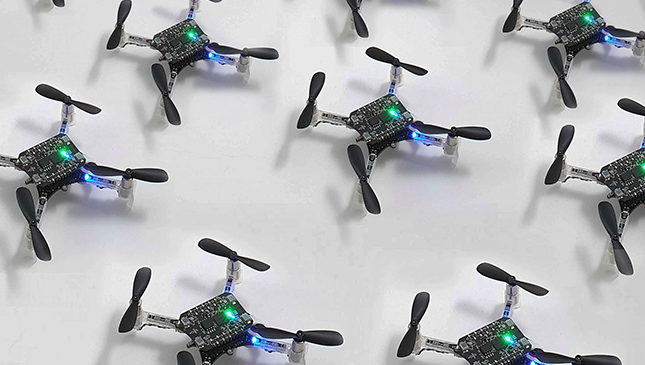
\includegraphics[height=4cm]{img/crazyflies.png}
\end{figure}

Seit kurzem steht am AerodrOHM eine Gruppe kleiner Micro-Drohnen (Crazyflies) zur Verfügung, die für koordinierte Formationsflüge programmiert werden können. Für einen dauerhaften und möglichst unterbrechungsfreien Betrieb des Schwarms ist eine zuverlässige Energieversorgung essentiell. Ziel dieser Arbeit ist die Entwicklung eines automatisierten Lade-Setups, bei dem die Drohnen selbstständig auf drahtlosen Ladepads landen und dort aufgeladen werden, ohne dass manuelle Eingriffe erforderlich sind.

Im ersten Schritt soll eine präzise Anflug- und Landeplanung entwickelt werden, die es den Drohnen ermöglicht, die Ladepads zuverlässig und positionsgenau anzufliegen. Dabei sind die begrenzte Onboard-Sensorik der Drohnen sowie die Positioniergenauigkeit des verfügbaren Lokalisierungssystems zu berücksichtigen. Auf der konstruktiven Seite sind die Ladepads mechanisch so zu gestalten, dass eine zuverlässige Kopplung mit den Drohnen gewährleistet ist. Schließlich soll die Ladeinfrastruktur in den Gesamtablauf integriert werden, sodass der Ladezustand überwacht und der Wechsel zwischen fliegenden und ladenden Drohnen automatisiert koordiniert werden kann.

\section*{Arbeitspakete}
\begin{itemize}[leftmargin=0.5cm]
    \setlength\itemsep{.1em}
    \item Einarbeitung in die Drohnenplattform und verfügbare Ladeinfrastruktur
    \item Entwicklung einer präzisen Anflug- und Landeplanung auf die Ladepads
    \item Konstruktive Anpassung und Fertigung mechanischer Komponenten (3D-Druck)
    \item Integration der Ladeinfrastruktur in den automatisierten Gesamtablauf
    \item Test und Evaluation des Lade-Setups im Flugraum des AerodrOHM
\end{itemize}

\section*{Voraussetzungen}
\begin{itemize}[leftmargin=0.5cm]
    \setlength\itemsep{.1em}
    \item Programmierkenntnisse in Python und/oder C++
    \item Erfahrung oder Interesse im Bereich Konstruktion, CAD oder Prototyping
    \item Freude an der praktischen Arbeit mit Hardware und am Aufbau von Prototypen
\end{itemize}

\vspace{0.5cm}
Das Thema kann nach Abstimmung als \textbf{Projekt-, Bachelor- oder Masterarbeit} bearbeitet werden.

\vfill
\textcolor{ohm_red}{\rule{\linewidth}{0.4mm}}
\textbf{\textcolor{ohm_red}{Labor für mobile Robotik}} \\
\begin{tabular}{@{}ll}
\textbf{Betreuer:} & Prof. Dr. Christian Pfitzner \\
\textbf{E-Mail:}   & \href{mailto:christian.pfitzner@th-nuernberg.de}{christian.pfitzner@th-nuernberg.de} \\
\end{tabular}

\end{document}
